\documentclass{article}
\usepackage[utf8]{inputenc}
\usepackage[ngerman]{babel}
\usepackage{pmboxdraw}

% Convenience improvements
\usepackage{csquotes}
\usepackage{enumitem}
\usepackage{amsmath}
\usepackage{amssymb}
\usepackage{mathtools}
\usepackage{tabularx}

% Proper tables and centering for overfull ones
\usepackage{booktabs}
\usepackage{adjustbox}

% Change page/text dimensions, the package defaults work fine
\usepackage{geometry}

\usepackage{parskip}

\usepackage{listings}

% Drawings
\usepackage{tikz}

% Adjust header and footer
\usepackage{fancyhdr}
\pagestyle{fancy}
\fancyhead[L]{Betriebssysteme --- \textbf{Übung 1}}
\fancyhead[R]{Laurenz Weixlbaumer (11804751)}
\fancyfoot[C]{}
\fancyfoot[R]{\thepage}
% Stop fancyhdr complaints
\setlength{\headheight}{12.5pt}

\newcommand{\R}{\mathbb{R}\ \\\ \{0\}}

\newcommand{\cmod}{\text{mod}}

\newcommand{\bO}{\text{O}}

\begin{document}

\section*{Aufgabe 1}

\begin{enumerate}
    \item Virtualbox starten.
    \begin{center}
        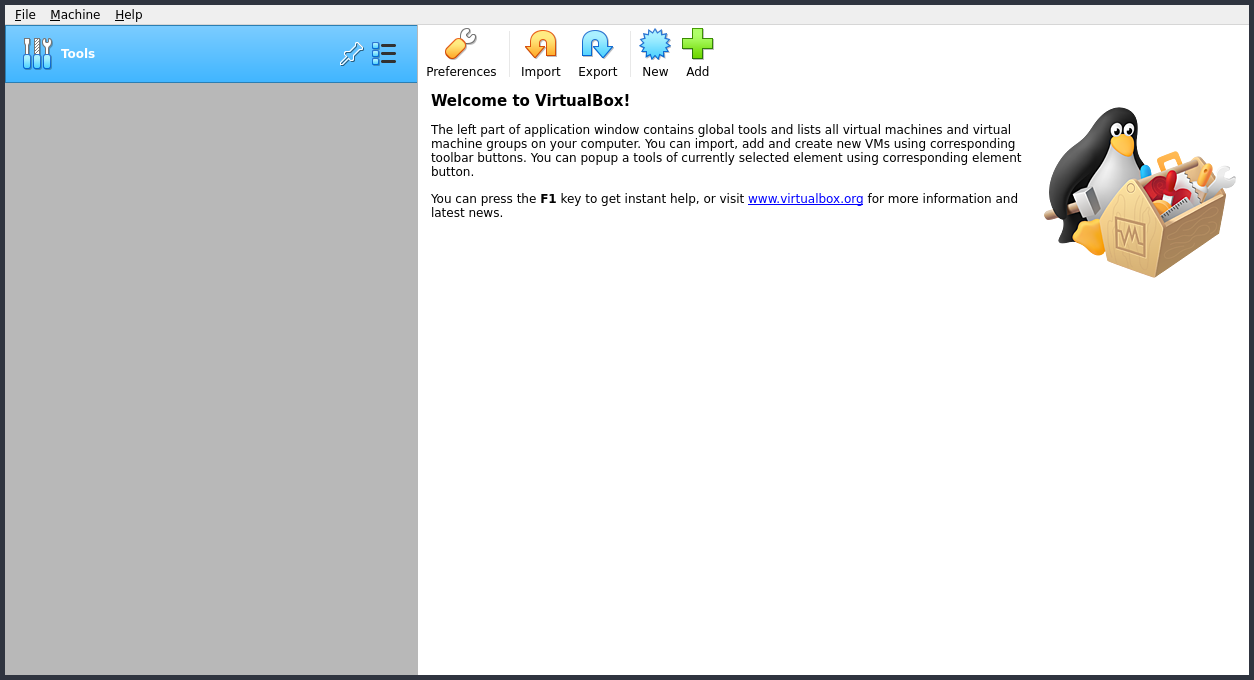
\includegraphics[width=0.7\textwidth]{01.png}
    \end{center}

    \item \emph{Import} klicken und die heruntergeladene .ova Datei auswählen.
    \begin{center}
        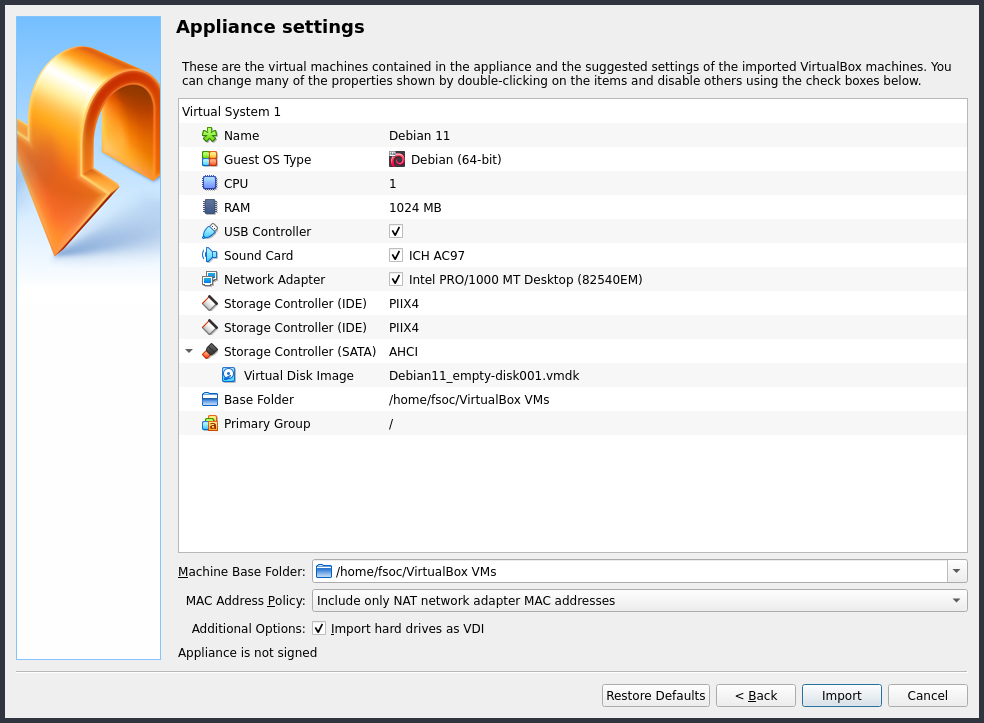
\includegraphics[width=0.7\textwidth]{02.png}
    \end{center}

    \item Einstellungen der importierten Maschine öffnen, auf den Reiter \emph{Storage} wechseln.
    \begin{center}
        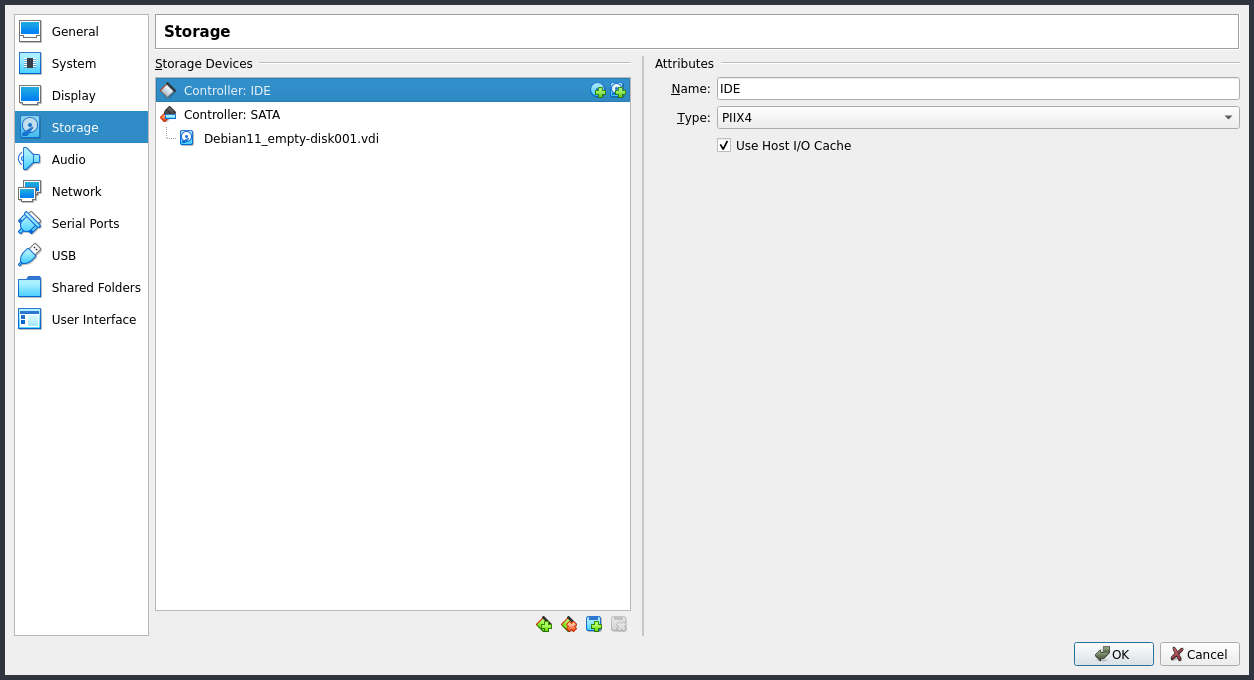
\includegraphics[width=0.7\textwidth]{05.png}
    \end{center}

    \item Unter \emph{SATA}, neues Medium hinzufügen. Nach Klick auf \emph{Add}, die heruntergeladene .iso auswählen.
    \begin{center}
        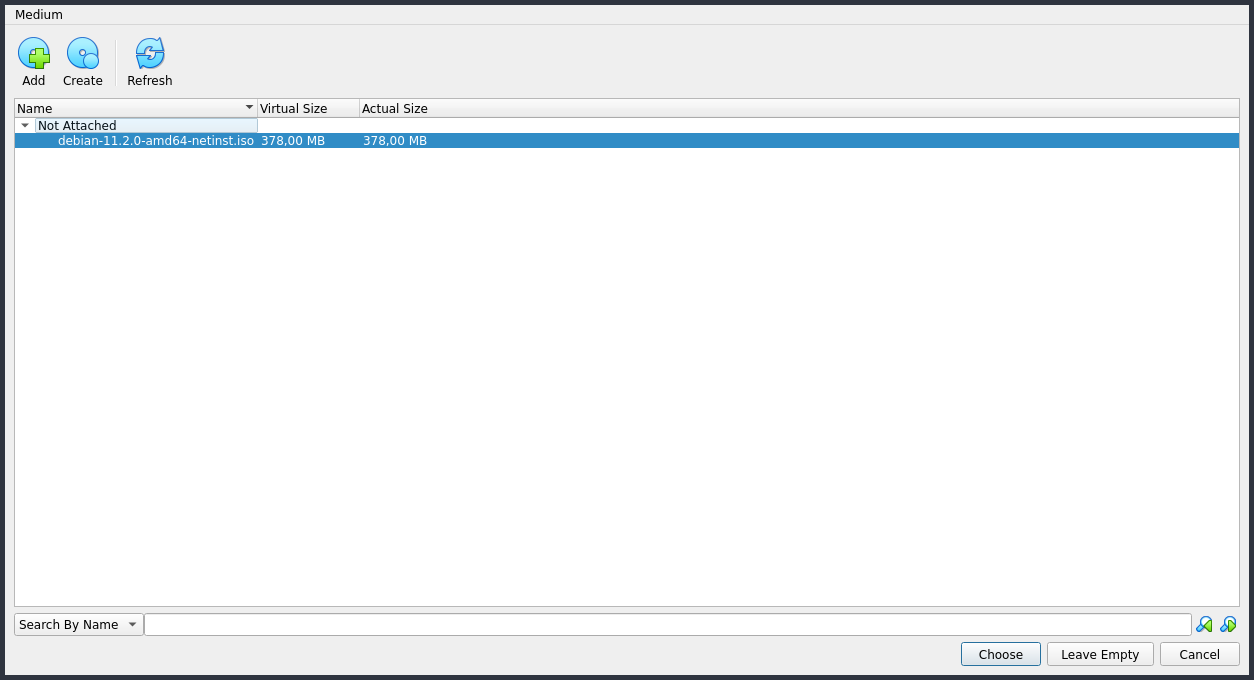
\includegraphics[width=0.7\textwidth]{06.png}
    \end{center}

    \item Klick auf \emph{Start}. Die defaults der graphischen Installation sind ausreichend, nur bei der auswahl des DE muss Xfce statt Gnome gewählt werden.
    \begin{center}
        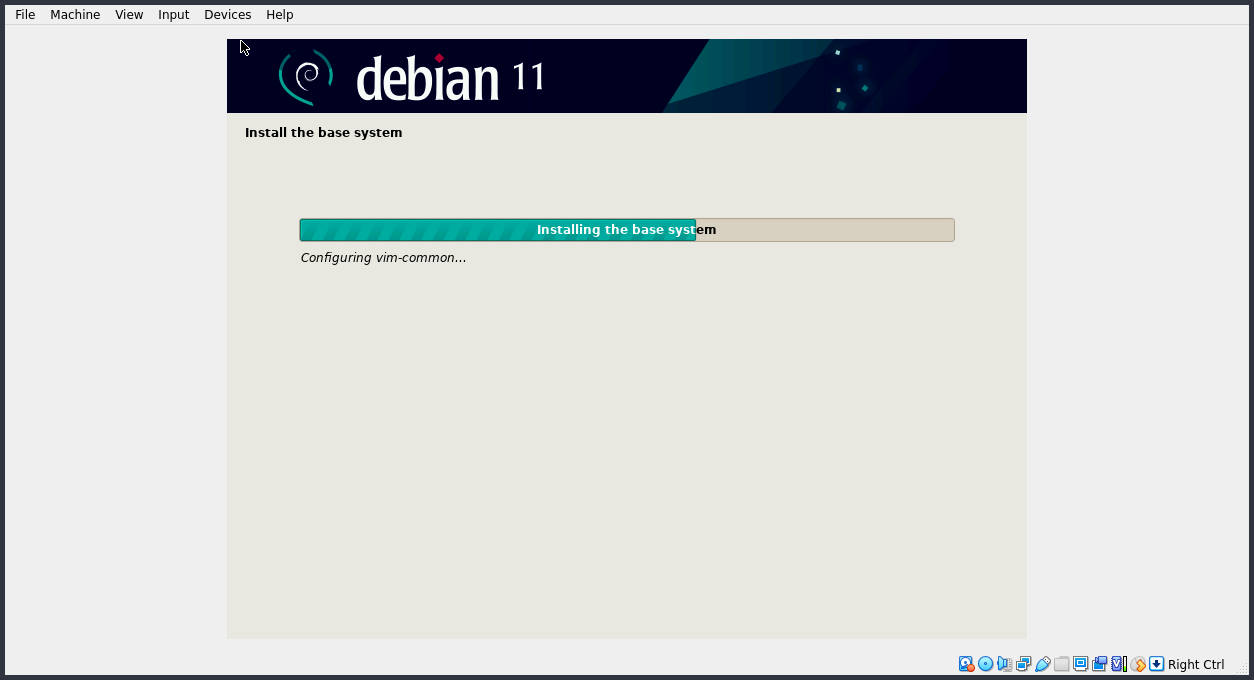
\includegraphics[width=0.7\textwidth]{08.png}
    \end{center}

    \item Fertig.
    \begin{center}
        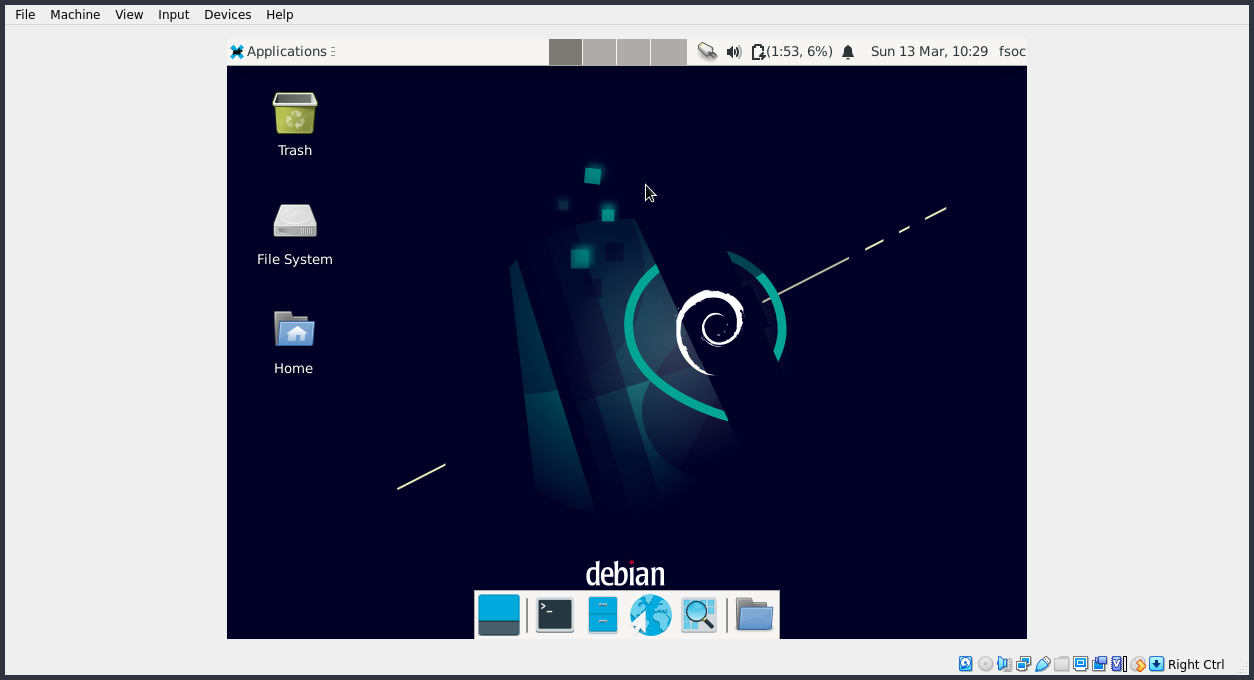
\includegraphics[width=0.7\textwidth]{09.png}
    \end{center}
\end{enumerate}

\section*{Aufgabe 2}

\begin{itemize}
    \item \begin{lstlisting}[breaklines]
$ cat /proc/version
Linux version 5.10.0-12-amd64 (debian-kernel@lists.debian.org) (gcc-10 (Debian 10.2.1-6) 10.2.1 20210110, GNU ld (GNU Binutils for Debian) 2.35.2) #1 SMP Debian 5.10.103-1 (2022-03-07)}
    \end{lstlisting}

    \texttt{cat file} gibt den Inhalt der Datei \texttt{file} aus. \texttt{/proc/version} beinhaltet informationen über die Version des laufenden Linux-Kernels und die Umgebung in und mit der er gebaut wurde.

    \item \begin{lstlisting}[breaklines]
$ uname -a
Linux debian 5.10.0-12-amd64 #1 SMP Debian 5.10.103-1 (2022-03-07) x86_64 GNU/Linux
    \end{lstlisting}

    \texttt{uname} gibt Systeminformationen aus. Der \texttt{-a} switch gibt alle bekannten Informationen aus. Obenstehend zu sehen sind der Kernelname (Linux), der Network Hostname (hier debian, kann vom Benutzer üblicherweise bei Installation geändert werden), das verwendete Kernelrelease (5.10.0-12-amd64), Kernelversionsinformationen (\#1 SMP Debian 5.10.103-1 (2022-03-07), Distributionsabhängig), Prozessortyp (x86\_64) und Betriebssystem (GNU/Linux).

    \item \begin{lstlisting}[breaklines]
$ lshw -short
WARNING: you should run this program as super-user.
H/W path        Device      Class       Description
===================================================
                            system      Computer
/0                          bus         Motherboard
/0/0                        memory      1GiB System memory
/0/1                        processor   Intel(R) Core(TM) i7-8550U CPU @ 1.80
/0/100                      bridge      440FX - 82441FX PMC [Natoma]
/0/100/1                    bridge      82371SB PIIX3 ISA [Natoma/Triton II]
/0/100/1.1                  storage     82371AB/EB/MB PIIX4 IDE
/0/100/2                    display     SVGA II Adapter
/0/100/3        enp0s3      network     82540EM Gigabit Ethernet Controller
/0/100/4                    generic     VirtualBox Guest Service
/0/100/5                    multimedia  82801AA AC'97 Audio Controller
/0/100/6                    bus         KeyLargo/Intrepid USB
/0/100/7                    bridge      82371AB/EB/MB PIIX4 ACPI
/0/100/b                    bus         82801FB/FBM/FR/FW/FRW (ICH6 Family) U
/0/100/d        scsi3       storage     82801HM/HEM (ICH8M/ICH8M-E) SATA Cont
/0/100/d/0.0.0  /dev/cdrom  disk        CD-ROM
/0/2                        input       PnP device PNP0303
/0/3                        input       PnP device PNP0f03
WARNING: output may be incomplete or inaccurate, you should run this program as super-user.
        \end{lstlisting}

        \texttt{lshw} gibt Informationen über die Systemhardware aus. Zu sehen sind etwa RAM, CPU, Netzwerkkarte, diverse andere Mikrochips, (virtuelle) Festplatte, etc.

        \item \texttt{pstree} gibt die dem System laufenden Prozesse als Baum aus. Durch den \texttt{-p} switch werden PIDs (Prozess IDs) mitausgegeben. \texttt{systemd} ist als Initialisierungssystem und Servicemanager mit PID 1 die Wurzel des Baums. Weitere nennenswerte Prozesse waren etwa \texttt{xfce4-terminal}, \texttt{NetworkManager}, \texttt{polkitd} (permission managemenet) und \texttt{lightdm} (desktop management).
        
        \item \texttt{lscpu} gibt Informationen über den Prozessor aus; etwa die Architektur, Byte-Reihenfolge, Anzahl der Kerne und Threads pro Kern, Geschwindigkeit der Kerne, Virtualisierungskapabilität, Cache-Größe, etc.
        
        \item \begin{verbatim}
               total        used        free      shared  buff/cache   available
Mem:           976Mi       562Mi        69Mi       7.0Mi       344Mi       270Mi
Swap:          974Mi        74Mi       900Mi
Total:         1.9Gi       637Mi       969Mi
        \end{verbatim}
        
        \texttt{free} gibt Aufschluss über den freien und verwendeten Arbeitsspeicher. Der \texttt{-h} switch erzeugt menschenlesbaren Output (Werte werden automatisch auf die größtmögliche Einheit skaliert), der \texttt{-t} switch erzeugt einen Zeile mit Gesamtwerten. Die Swap-Spalte repräsentiert hier jenen Teil der Festplatte der zum Ablagern von selten verwendeten Speicherpages verwendet wird (oder potentiell für eine Hibernate Funktionalität, etc.).

        \item \begin{verbatim}
$ uptime -s
2022-03-13 11:01:14
        \end{verbatim}

        \texttt{uptime} gibt Informationen darüber, seit wann das System läuft. Der switch \texttt{-s} zeigt diese Information in Form des Startdatums, was die Information abhängig von der konfigurierten Zeitzone macht.
\end{itemize}

% cat /proc/version
% Linux version 5.10.0-12-amd64 (debian-kernel@lists.debian.org) (gcc-10 (Debian 10.2.1-6) 10.2.1 20210110, GNU ld (GNU Binutils for Debian) 2.35.2) #1 SMP Debian 5.10.103-1 (2022-03-07)

% uname -a

% lshw -short

% pstree -p

% lscpu

% free -ht

% uptime-s

\end{document}
